\documentclass{standalone}

\usepackage{tikz}
\usepackage{tikzpeople}
\usetikzlibrary{shapes.geometric}

\tikzset{database/.style={
		cylinder,
		aspect=1,
		draw,
		thick,
		fill,
		shape border rotate=90,
		minimum height=1.5cm,
		left color=green!30,
		right color=green!30,
		middle color=green!30,
		minimum width=2cm,
		path picture={
			\draw[black, thick] let \p1=($(path picture bounding box.north east)-(path picture bounding
			box.south west)$) in 
			foreach \XX in {1,2,3}  {([yshift=-\XX*\y1/4]path picture bounding box.north west) 
				arc(180:360:\x1/2 and 0.25*\x1/2)};
		}}}

\begin{document}
			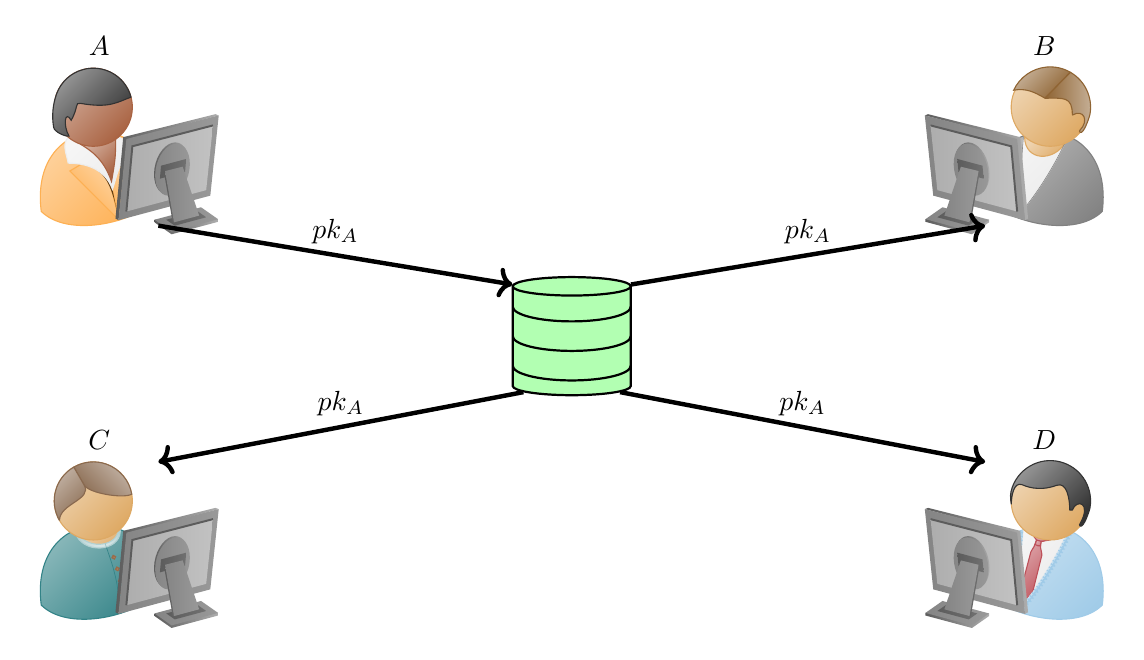
\begin{tikzpicture}
				\node[alice, monitor, label=$A$, minimum size=1.5cm] (Alice) at (0,0) {};
				\node[bob, mirrored, monitor, label=$B$, minimum size=1.5cm] (Bob) at (12,0) {};
				\node[charlie, monitor, label=$C$, minimum size=1.5cm] (Charlie) at (0,-5) {};
				\node[dave, mirrored, monitor, label=$D$, minimum size=1.5cm] (Dave) at (12,-5) {};
				\node[database,minimum size=1.5cm] (S) at (6,-2.5) {};
				
				\draw[->,ultra thick] (Alice.south east) -- (S.north west) node[midway,above] {$pk_{A}$};
				\draw[->,ultra thick] (S.south east) -- (Dave.north west) node[midway,above] {$pk_{A}$};
				\draw[->,ultra thick] (S.north east) -- (Bob.south west) node[midway,above] {$pk_{A}$};
				\draw[->,ultra thick] (S.south west) -- (Charlie.north east) node[midway,above] {$pk_{A}$};
			\end{tikzpicture}
\end{document}
